%%%%%%%%%%%%%%%%%%%%%%%%%%%%%%%%%%%%%%%%%%%%%%%%%%%%%%%%%%%%%%%%%%%%%%%%
%                                                                      %
%     File: Thesis_Implementation.tex                                  %
%     Tex Master: Thesis.tex                                           %
%                                                                      %
%     Author: Andre C. Marta                                           %
%     Last modified :  2 Jul 2015                                      %
%                                                                      %
%%%%%%%%%%%%%%%%%%%%%%%%%%%%%%%%%%%%%%%%%%%%%%%%%%%%%%%%%%%%%%%%%%%%%%%%

\chapter{Proposed Work}
\label{chapter:implementation}

The proposed project consists in the development of a Yolov3 CNN application for
Deep Versat, with focus on the convolutional layer, that represents the majority
of computations in CNNs.

This involves the design of a set of acceleration datapaths for Deep Versat,
which, in turn, may require the improvement of the existing FU set. The overall
goal is to accelerate the execution of the application up to 30 images per
second in order to achieve video speed.

% intro to several sections

\section{Yolov3 Software Modeling}
\label{sec:yolov3_baseline}
The Yolo networks use Darknet~\cite{darknet13}, an open source neural network in
C and CUDA, which does not have support for reduced precision
operands. Therefore, the development of a code base that facilitates the
evaluation of the Yolov3 network in terms of operand precision becomes a
requirement.

This evaluation is necessary to verify the accuracy of the network with reduced
precision operands and to measure the ranges of the activations at each
layer. Only with this analysis it is possible to implement an effective
quantization based on DFP (section~\ref{sec:quantization}), which is necessary
for deep networks.


\section{Baseline Hardware System}
\label{sec:hw_baseline}
In order to establish a baseline for the performance of the Deep Versat, the
system presented in Fig.~\ref{fig:baseline_hw_system} will be used. The
architecture uses as base the system in~\cite{VMario:Deep_Versat}.

The main difference from the system in~\cite{VMario:Deep_Versat} is the addition
of the DMA connection between the Deep Versat and the external memory. As
discussed in~\ref{sec:Versat_controller}, this change frees the host system
during data transfers.

A RISC-V processor is used as the host and controller for Deep Versat. This soft
processor treats each other block in the system as a memory mapped
peripheral. The processor is also tasked to execute the parts of the application
that are not accelerated by the Deep Versat.

The UART block is useful in development for debugging purposes, as it is a
practical way to receive feedback from the system into a console on an external
computer.

Deep Versat has been programmed with a convolutional layer for accelerating a
hand written digit recognition application~\cite{VMario:Deep_Versat}. This
implementation uses Versat's current set of FUs, which are reconfigured many
times to form datapath configurations as discussed in~\ref{sec:Deep_Versat}.

With this implementation it is possible to both verify the correct functioning of
the system and all its components, as well as establishing a baseline in terms
of performance for convolution acceleration.

\begin{figure}[!htb]
	\centering
	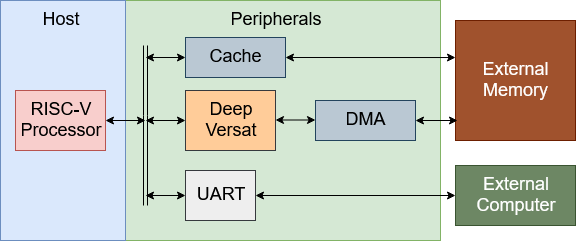
\includegraphics[width=0.6\textwidth]{Figures/baseline_HW_system.png}
	\caption[Caption for figure in TOC.]{Baseline hardware system}
	\label{fig:baseline_hw_system}
\end{figure}
%FIX o que liga o risc-v a memoria externa é uma cache e não um dma. Não existe Program Memory, é a cache. (FIXED)

\section{Datapath Proposal for Convolutional Layers}
\label{sec:planned_datapath_for_conv_layers}
The acceleration of convolutional layers will start with the proposal of a
datapath architecture, based on the analysis
in~\ref{sec:Datapath_Optimizations}. The accelerator presented
in~\ref{sec:proposed_accelerator} is a promising starting point for the
architecture.

The designed datapaths may require the development of new of FUs or tweaking of
the existing ones. There is then the challenge of mapping the convolution
datapaths into the Deep Versat architecture using the modified FU set.  After
that, the convolution layer can be tested and compared with the baseline
results. The work reported in this section is the main focus of the project and
is expected to be the most time consuming task.

\section{Experimental Validation with Yolo Networks}
\label{sec:experimental_yolo_validation}
With a new Convolutional Layer tested and working properly, the next test is to
execute the Tiny-Yolov3 network (section~\ref{sec:tiny-yolov3}) on the
system. This represents an intermediate step due to the reduced requirements of
this network, when compared with the full Yolov3. As a general goal for the
project, processing 30 images per second would be ideal, although this objective
may not be achieved.


%FIX: Não percebi porque é preciso desenvolver uma FU para conv. Já existe o MAC tal
%como explicaod no Alg1. O que podemos ter de mexer é nas AGUs para aumentar o
%numero de loops executados no Deep Versat


\section{Work Calendarization}
\label{sec:tasks_GANT}
In Fig.~\ref{fig:tasks_callendar} it is presented a GANT chart outlining the
calendarization of the planned work.


%FIX: altera o planeamento de acordo uma vez que não vejo a tarefa de desenhar uma FU como dominante.

\begin{figure}[!htb]
	\centering
	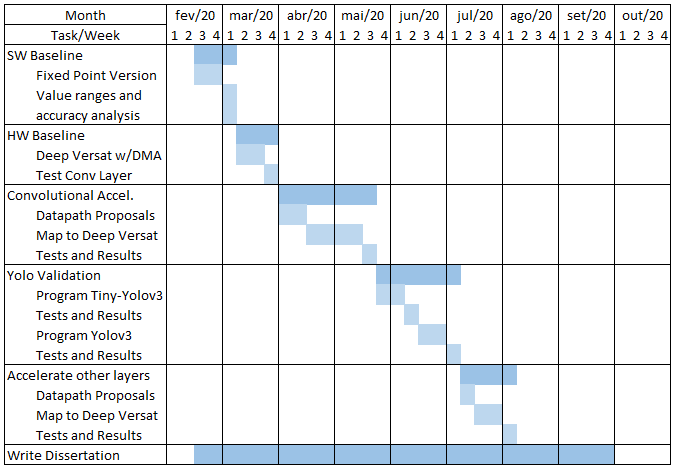
\includegraphics[width=0.95\textwidth]{Figures/dummy_GANT.png}
	\caption[Caption for figure in TOC.]{Work Planning}
	\label{fig:tasks_callendar}
\end{figure}


%\begin{itemize}
%	\item Proposed Methodologies
%	\subitem Outline of base system
%	\subitem PE in Versat architecture
%	\subitem General PE architecture proposal
%	\item Expected Results
%	\subitem Target performances and goals (accuracy, fps, networks)
%	\item Work planning table (GANT)
%\end{itemize}


